\documentclass[a4paper,12pt]{report}
\usepackage[T1]{fontenc}
\usepackage[utf8]{inputenc}
\usepackage[francais]{babel}
\usepackage[usenames,dvipsnames,svgnames,table]{xcolor}
\usepackage[colorlinks,linkcolor={blue!30!black},citecolor={blue!50!black},urlcolor={blue!80!black}]{hyperref}
\usepackage{amsmath,array,graphicx,caption,lmodern,subcaption,tikz,url,xspace,wrapfig}
\usepackage{textcomp,rotating,epic,eepic,pdfpages}
\usepackage[top=2cm,left=2.5cm,right=2.5cm,bottom=2cm]{geometry} % Géométrie de la page, modifier selon le besoin
\usepackage[babel=true,kerning=true]{microtype}

\addto{\captionsfrench}{\renewcommand{\abstractname}{Introduction}}
\pdfsuppresswarningpagegroup=1
\date{}
\title{Rapport de Stage d'Application}
\author{Félix Piédallu}

\newcommand{\HeT}{$^3$He\xspace}
\newcommand{\HeQ}{$^4$He\xspace}


\begin{document}
\nocite{*}
\pagenumbering{gobble}  % Pas de numérotation
\begin{titlepage}
    \vspace*{-10px}
    
\includegraphics[height=80px]{Images/logo_phelma.pdf}
    \vspace*{-80px}
\begin{flushright}
    \vspace*{-30px}
    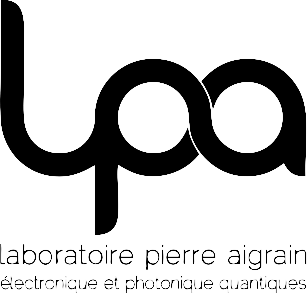
\includegraphics[height=100px]{Images/logo_lpa.png}
\end{flushright}

\vspace*{0.5cm}
\begin{center}
\rule{\linewidth}{0.5mm}\\[0.4cm]
{\huge{\bfseries Rapport de Stage d'Application}\\[0.4cm]
Mise en place d'une expérience à très basse température et étude d'effets quantiques dans des systèmes nanométriques\\[0.4cm]}
\rule{\linewidth}{0.5mm}\\[0.5cm]

\LARGE{\textsc{Félix Piédallu}}\\[0.7cm]
\large{\textsc{Filière PNS 2014-2015}}\\[2cm]

\Large{Au sein de l'équipe HQC}\\[1cm]

\includegraphics[width=0.4\textwidth]{Images/logo_HQC.pdf}\\[1cm]

\large{Sous la direction de Takis \textsc{Kontos} et Laure \textsc{Bruhat}}\\[2cm]


\end{center}
\end{titlepage}

\tableofcontents        % Table des matières avec liens, générée automatiquement.
\newpage
\pagenumbering{arabic}  % Numérotation de retour !


% Remerciements
\vspace*{\stretch{1}}
\begin{center}
\textsc{\Large Remerciements}
\\
\vspace{0.5cm}
Je tiens à remercier Takis Kontos et Laure Bruhat pour m'avoir accueilli au sein de l'équipe HQC, ainsi que pour m'avoir encadré durant ce stage. De plus, je souhaite remercier l'ensemble des membres de l'équipe, avec lesquels j'ai pu échanger sur leurs projets de recherche. Enfin, je souhaite remercier Phelma Grenoble-INP pour m'avoir donné l'opportunité de réaliser ce stage.
\end{center}
\vspace*{\stretch{3}}


\chapter*{Hybrid Quantum Circuits}
L'équipe HQC fait partie du Laboratoire Pierre Aigrain, le laboratoire de l'ENS Ulm spécialisé dans la physique de la matière condensée et la physique mésoscopique.

Elle regroupe autour de Takis Kontos et Audrey Cottet plusieurs doctorants : Matthieu Baillergeau, Matthieu Desjardins, Matthieu Dartiailh et Laure Bruhat, avec qui j'ai essentiellement travaillé durant mon stage.\newline

L'équipe se concentre sur l'utilisation des nanotubes de carbone, en tant que double puits quantique ou qu'atome macroscopique (atome artificiel).

Le nanotube de carbone est placé dans une cavité résonnante dont on fait varier les paramètres, et donc la fréquence de résonnance. Les sujets de recherche sont donc essentiellement concertés autour de la spintronique et du transport quantique dans de tels milieux.

L'équipe met donc en place le modèle théorique d'une part, et s'occupe de la fabrication des échantillons et de la mise en place de l'expérience.\newline

Le laboratoire est équipé d'un cryostat à Hélium3 (Oxford Heliox VL), d'un cryostat à dilution (Kelvinox Oxford MX250) et d'un cryostat à dilution sèche (Cryoconcept Cryofree), sur lequel j'ai travaillé dans le cadre de mon stage.





\chapter*{Introduction} % Contexte du stage
\addcontentsline{toc}{chapter}{Introduction}

Laure Bruhat a entamé depuis plus de deux ans une thèse portant sur la séparation des paires de Cooper intriquées dans une cavité micro-ondes et le transport quantique. Pour ce faire, elle a mis en place une expérience dans un cryostat à dilution sèche, fourni par CryoConcept.
\par
\begin{figure}[h]
    \begin{center}
        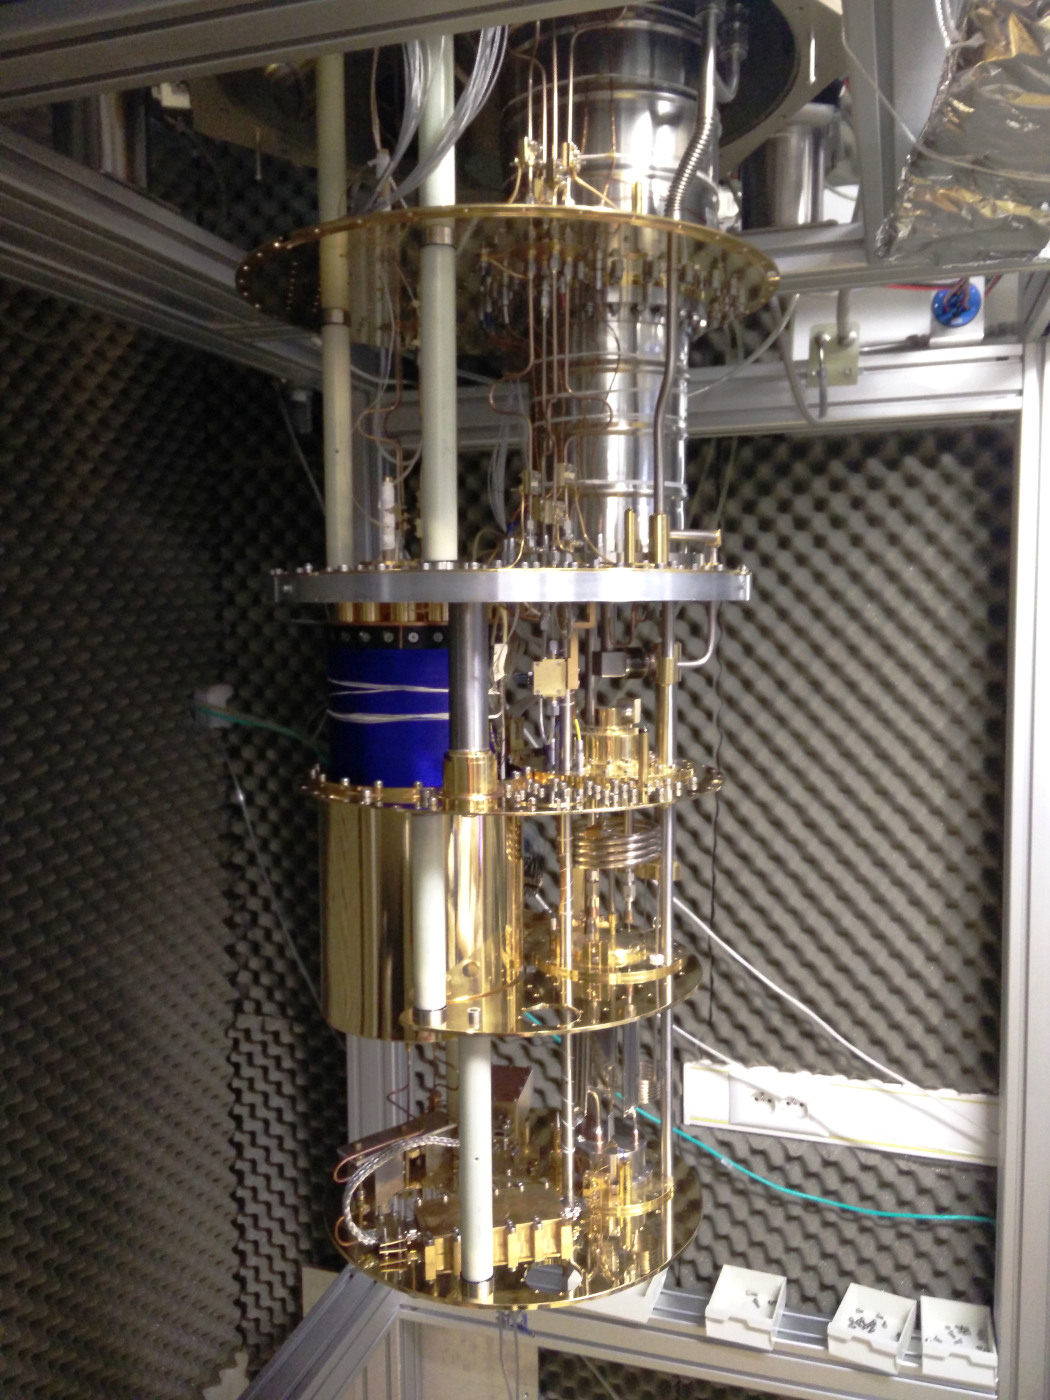
\includegraphics[height=0.7\textwidth]{Images/Global.jpg}
        \caption{Le cryostat ouvert avec la bobine (bleue)}
        \label{photo_separateur_nanotube}
    \end{center}
\end{figure}


Ce cryostat étant "spacieux", Takis Kontos et Laure Bruhat ont décidé d'y rajouter une expérience. Celle-ci serait placée au sein d'un champ magnétique, généré par une bobine installée dans le cryostat. Cette expérience pourra donc permettre d'étudier l'influence du champ magnétique ($\sim$700mT) sur la séparation des paires de Cooper.\newline

Mon travail consiste donc à comprendre l'ensemble du fonctionnement du cryostat, et à câbler la seconde expérience, de la fabrication des câbles à leur caractérisation et leur mise en place dans le cryostat. Il consiste aussi à mettre à froid pour les divers tests du cryostat après la mise en place de la bobine.


\chapter{L'expérience}


\section{Interaction d'électrons et de photons dans un nanotube de carbone}
\subsection{Un milieu 1D (nanotube)}

\subsection{Une cohérence spatiale (atome artificiel)}
$\rightarrow$ Pas de bruit ambiant $\rightarrow$ cryostat

\subsection{L'interaction Électrons/Rayonnement Gigahertz}
$\rightarrow$ Contrôle excellent du signal envoyé $\rightarrow$ câbles coaxiaux les plus parfaits possibles

\subsection{Quelques exemples d'expériences}
\begin{itemize}
    \item Cooper Pair Splitter
    \item Couplage Champ électrique/Trajectoire/Spin
\end{itemize}

\section{Fabrication des nanotubes de Carbone}

\section{Utilisation du champ magnétique}


\chapter{Le cryostat à dilution}
Afin d'accéder à des températures de l'ordre que la dizaine de milliKelvins, l'expérience est située dans un cryostat à dilution sèche.
\section{Principe d'un cryostat à dilution}
\begin{figure}[h]
  \begin{center}
    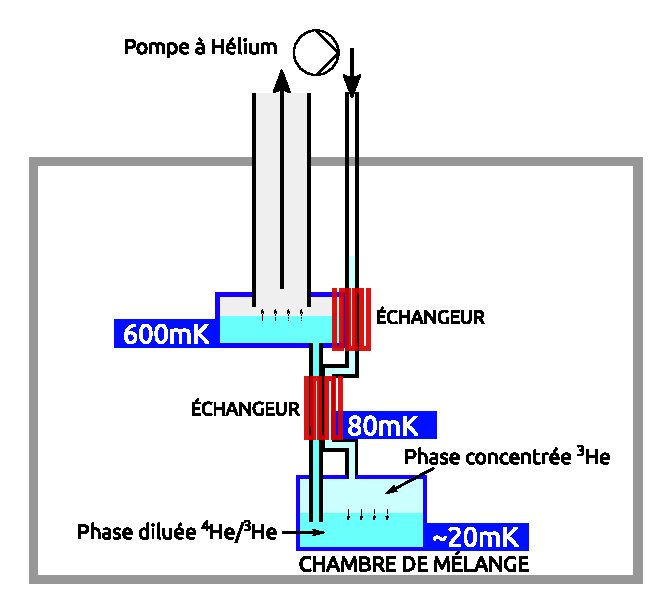
\includegraphics[width=0.6\textwidth]{Images/Cryostat_Schema.pdf}
    \qquad
    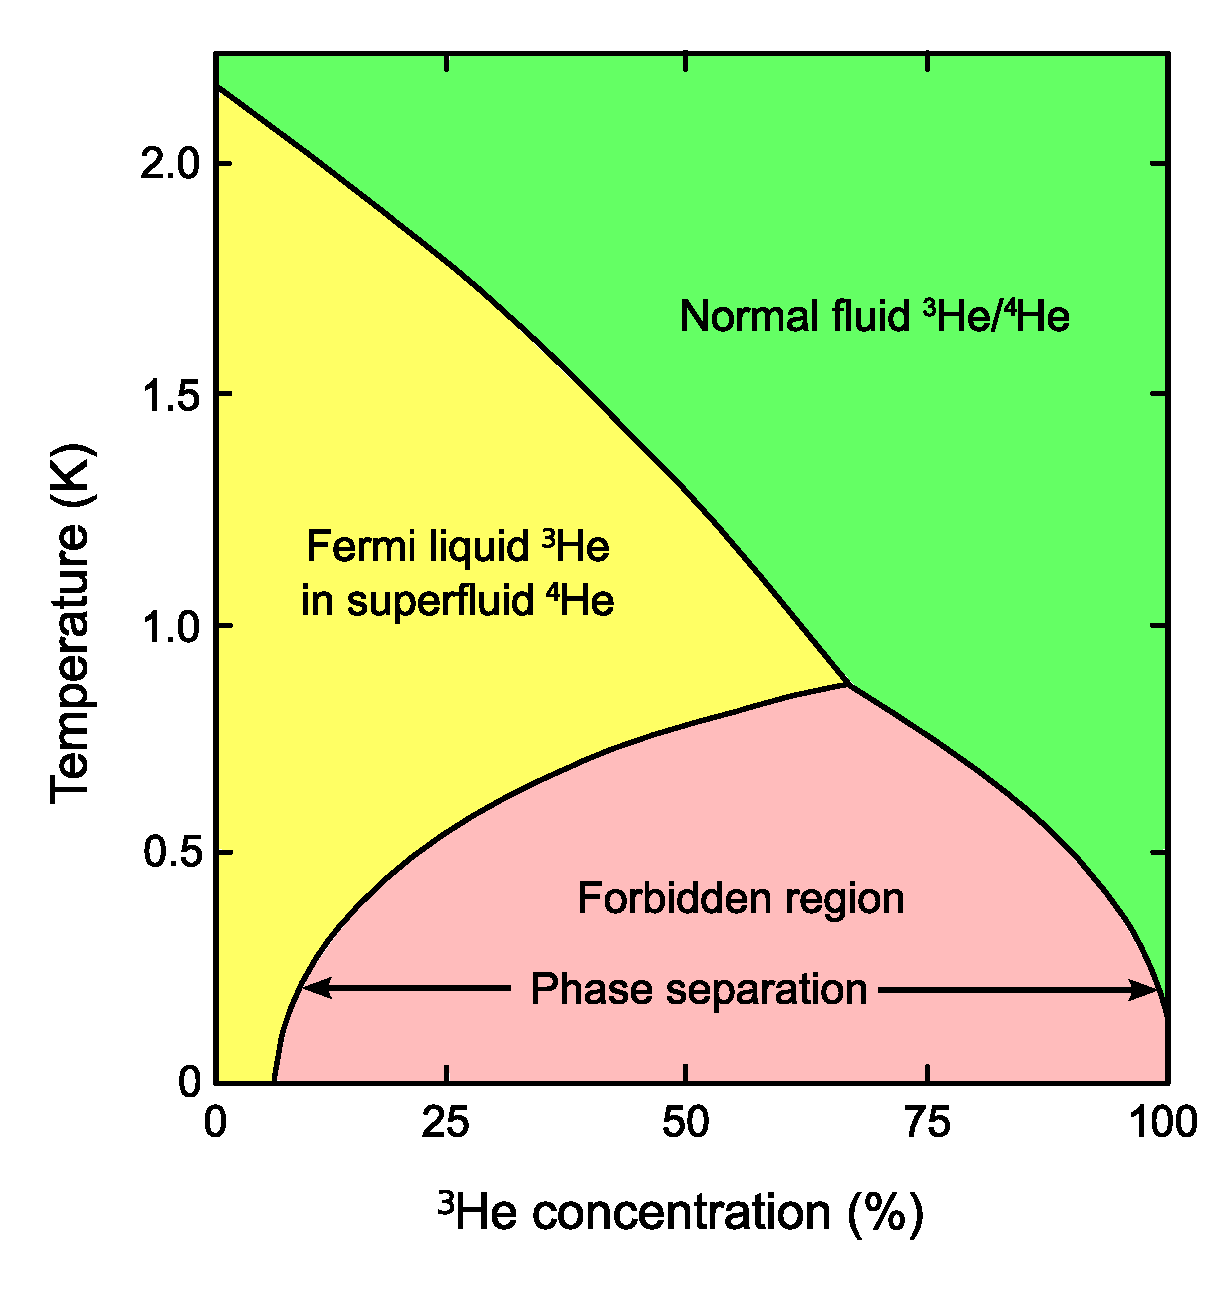
\includegraphics[width=0.33\textwidth]{Images/Helium_phase_diagram.pdf}
    \caption{Schéma du cryostat à dilution et diagramme de phase du mélange d'Hélium}
  \end{center}
\end{figure}
Le cryostat à dilution est basé sur certaines propriétés du mélange des isotopes d'Hélium \HeT et \HeQ.
\newline

Prenons un mélange équilibré liquide \HeT/\HeQ(donc pré-refroidi à 1K) ; l'\HeQ étant le plus lourd, il tombe au fond et l'\HeT flotte au-dessus.

Ensuite, du point de vue des interactions quantiques dans chacun des liquides, on remarque que les interactions pour l'atome d'\HeT sont plus faibles que pour l'\HeQ : les premiers vont descendre dans la phase \HeQ, mais pas l'inverse.
\newline

On se trouve donc en présence de deux phases: celle, plus légère, d'\HeT pur, et celle de mélange \HeT/\HeQ.
Enfin, les atomes d'\HeT sont des Fermions, et le principe d'exclusion de Pauli s'y applique: la solubilité de l'\HeT dans l'\HeQ sera limitée aux environs de \{6,6\% \HeT, 93.4\% \HeQ\}.
\newline

Lorsqu'on pompe de l'\HeT de la phase diluée vers la phase pure, une pression osmotique va apparaître à l'interface des deux phases: l'\HeT va alors se dissoudre dans la phase diluée. Or cette réaction est endothermique, et ceci fournit la puissance calorifique au cryostat.

Ceci se passe au niveau de la chambre de mélange.\newline

Lorsque la pompe diminue la pression dans cette chambre de mélange, la phase diluée va monter jusqu'au réservoir supérieur. Ici, la température est aux alentours de 600-800mK et la pression de $\sim$10Pa.

L'\HeT va essentiellement s'évaporer du mélange. En effet, il a une pression partielle bien plus évelée que l'\HeQ, qui lui va en grande partie rester confiné dans le réservoir et dans la chambre de mélange.
\newline

La vapeur va alors passer par la pompe (à température ambiante), être refroidie pour revenir jusqu'à la chambre de mélange où la pression osmotique entre les deux phases va augmenter d'autant plus: de l'\HeT va alors passer dans la phase diluée en refroidissant le cryostat, et recommencer le processus. \newline

Les échangeurs thermiques permettent à l'\HeT réinjecté d'être remis à basse température pour ne pas réchauffer l'ensemble du cryostat. Cela permet aussi d'augmenter la température dans le réservoir supérieur et permettre à l'\HeT de s'évaporer.

\section{Cryostat sec: Principe du tube à gaz pulsé}
Le mélange doit être pré-refroidi avant d'être injecté dans le cryostat.\newline
La plupart des cryostats utilisent un bain d'azote liquide à 77K qui permet aussi de nettoyer le mélange des impuretés, un bain d'\HeQ liquide à 4,2K, puis un bain d'\HeQ liquide à faible pression à 1K (diminuer la pression de l'\HeQ permet d'abaisser son point de condensation).

Ces derniers bains nécessitant un apport d'\HeQ, il peuvent être remplacé par un tube à gaz pulsé, d'où l'appellation de cryostat sec (mis à part le bain d'azote liquide qui est à l'extérieur du cryostat).

Un tube à gaz pulsé fonctionne selon un cycle proche du cycle de Stirling, grâce à un piston et un compresseur. Ceux-ci engendrent des vibrations importantes, qui pourraient empêcher toute mesure dans le cryostat. C'est pour cela que le tube pulsé est séparé du cryostat.

\begin{figure}[ht]
    \begin{center}
        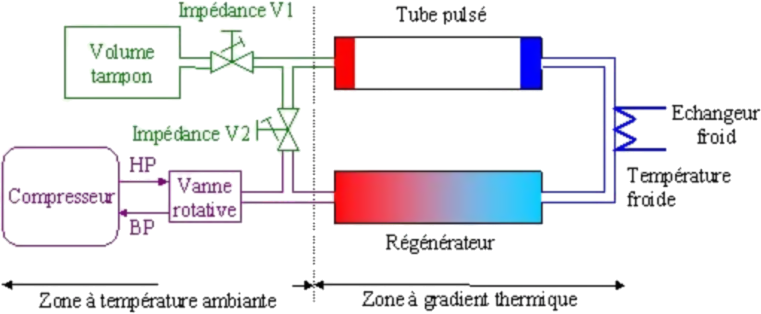
\includegraphics[width=0.75\textwidth]{Images/Cryostat_PulseTube_Schema.png}
        \caption{Schéma du tube à gaz pulsé}
    \end{center}
\end{figure}


\begin{figure}[ht]
    \begin{center}
        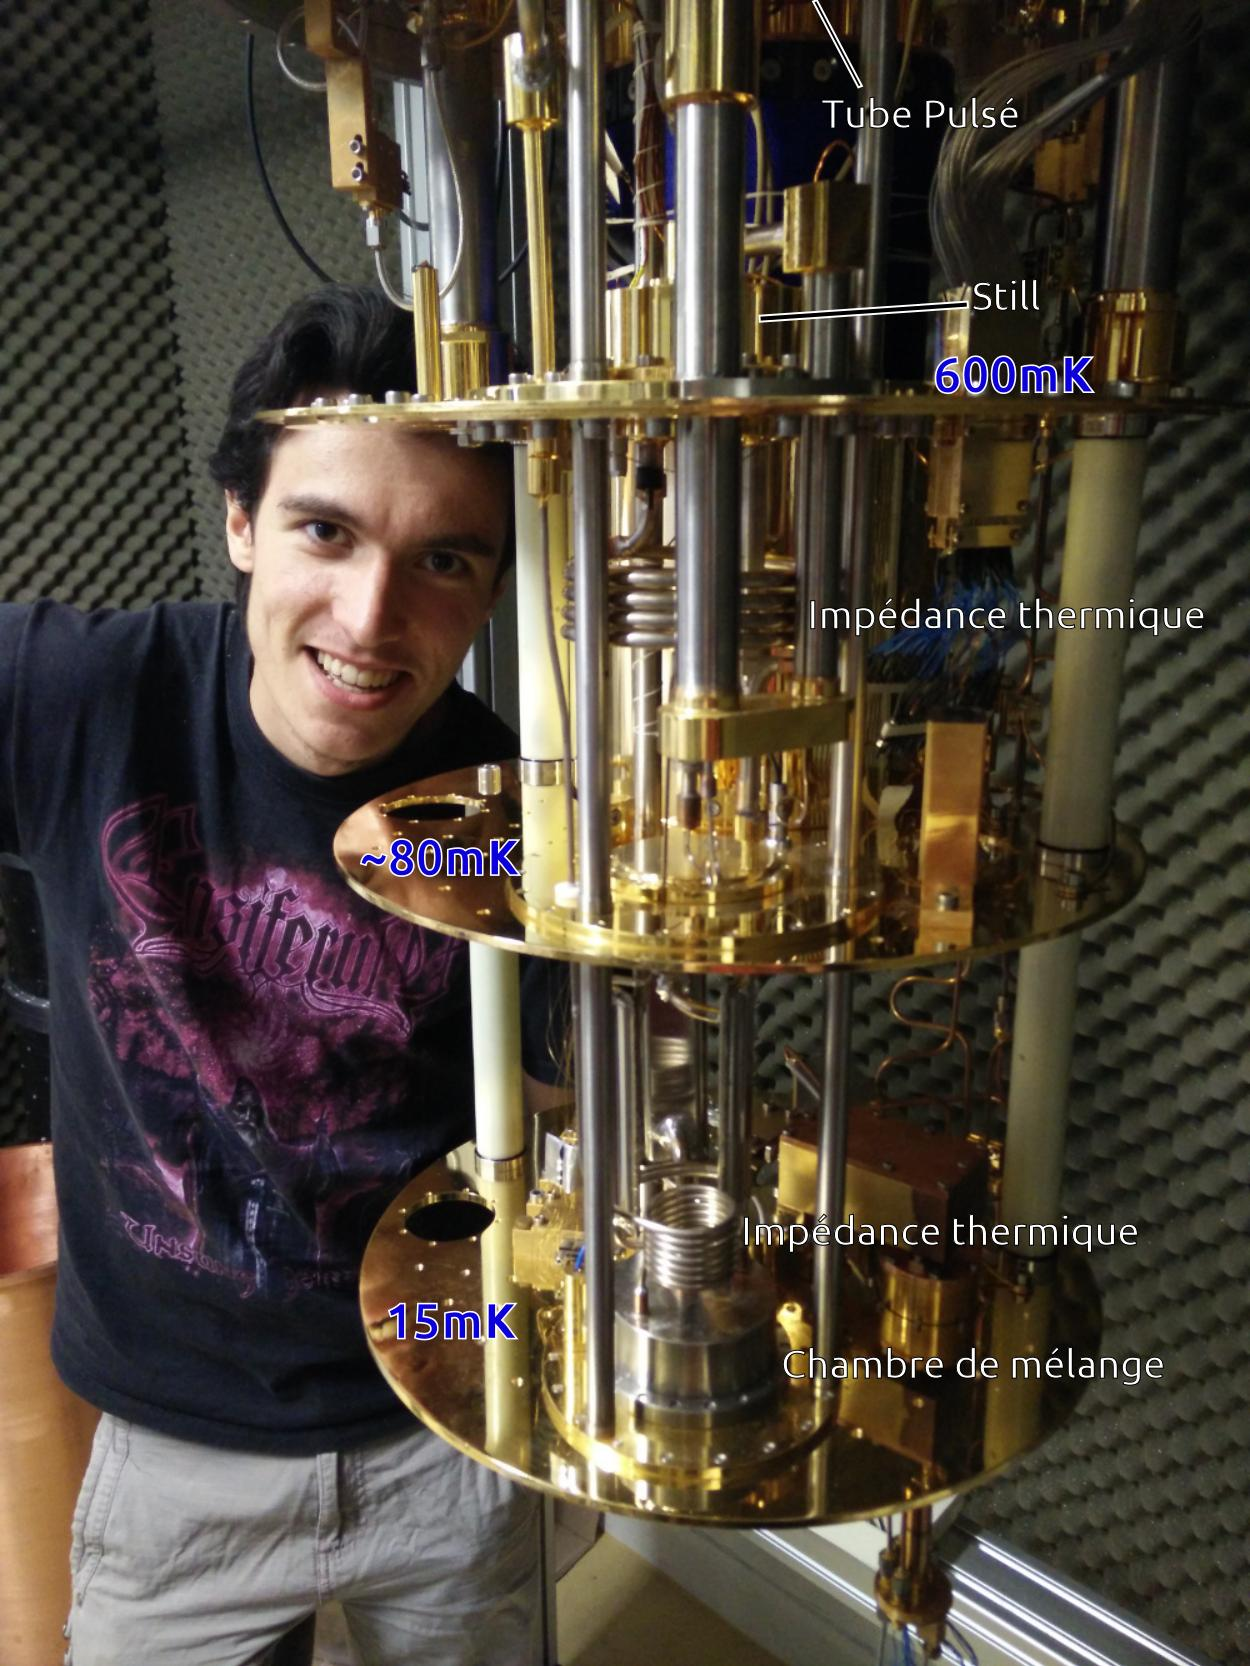
\includegraphics[width=0.75\textwidth]{Images/PhotoCryostat}
        \caption{Organisation du cryostat à dilution sèche}
    \end{center}
\end{figure}


\chapter{Le câblage DC et RF}
\vspace*{-0.5cm}
Le câblage du cryostat consiste en deux parties: 
\paragraph*{Les câbles DC: }ils véhiculent les signaux continus. Au nombre de 17, ils sont thermalisés à chaque étage pour limiter le bruit thermique.
\paragraph*{Les câbles coaxiaux: }les deux grilles rapides, le signal d'entrée et le signal de sortie. Ils font l'objet de beaucoup d'attention, afin d'avoir les meilleures mesures possibles.

\vspace*{0.2cm}
\begin{figure}[h]
    \begin{center}
        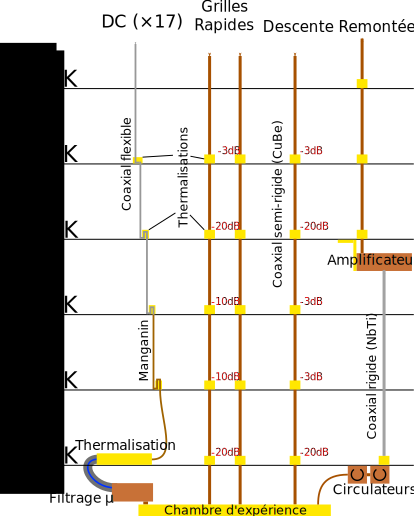
\includegraphics[width=0.7\textwidth]{Images/Cablage_schema}
        \caption{Schéma de câblage de l'expérience}
        \label{cablage_schema}
    \end{center}
\end{figure}




\section{Choix des matériaux}
Parlons tout d'abord des câbles de descente. Ceux-ci véhiculent le bruit thermique d'étage en étage, ce que nous voulons limiter au maximum.

Nous faisons donc le choix de câbles atténuant le signal afin de limiter l'apport de bruit. Ceci permet en plus de limiter les ponts thermiques entre étages dûs à la conductivité des câbles.
\newline

Les câbles DC sont alors:
\begin{itemize}
    \item des câbles coaxiaux souples entre 300K et 800mK, peu résistifs (le signal est suffisant pour avoir un bon rapport signal/bruit)
    \item des câbles de Manganin, très résistifs ($\sim45\Omega/m$), jusqu'à 20mK (l'étage le plus froid)
    \item des câbles peu résistifs ($\sim0.4\Omega/m$) jusqu'à la chambre d'expérience
    \newline
\end{itemize}

et les câbles RF coaxiaux semi-rigides de descente sont:
\begin{itemize}
    \item en Cuivre-Béryllium, thermalisé à chaque étage, jusqu'à 20mK. Le CuBe est beaucoup plus résistif que le Cuivre.
    \item en Cuivre jusqu'à la chambre d'expérience
\end{itemize}

Les câbles sont cintrés en "U" entre chaque étage, afin de limiter le passage des radiations au maximum. Ceci permet de plus d'avoir une certaine souplesse dans les câbles pour les connecter sans trop de difficultés.\newline

Enfin, on rajoute à chaque étage un atténuateur (valeur en rouge sur le schéma). Ceci permet d'envoyer en amont du cryostat un signal très fort, qui détruirait les échantillons, pour avoir dès le départ un rapport signal/bruit très bon.


\paragraph*{Pour le câble de remontée,}on raisonne différemment: il faut atténuer le signal le moins possible, jusqu'à l'amplificateur haute fréquence qui est situé à 4K (sa température nominale de fonctionnement). Un câble rigide de Niobium-Titane est alors utilisé.

Afin de limiter le "retour" de signal de l'amplificateur par ce câble, on thermalise deux circulateurs à 20mK. On utilise des câbles de Cuivre pour les connexions avec la chambre d'expérience.






\section{Thermalisation électronique}
Une grande partie du bruit provient de la température électronique. Si les câbles ne sont pas bien thermalisés, on risque de ne mesurer qu'un bruit à 300K.
\newline

Les câbles coaxiaux sont thermalisés à chaque étage du cryostat par des pinces, reliées par des câbles de cuivre jusqu'aux platines du cryostat. L'ensemble des pièces est bien sûr doré pour avoir les meilleurs contacts thermiques possibles ; les pores des parois en contact sont bouchées par de l'Apiezon N, à l'instar de la pâte thermique de nos processeurs.
\newline

Les câbles DC sont thermalisés à chaque étage par des presses dorées grâce à de la Stycast. Cette époxy permet une très bonne thermalisation des câbles fins aux presses dorées et montées sur les platines du cryostat.

Une thermalisation s'effectue aussi au niveau du boîtier de thermalisation où les câbles font des méandres afin d'assurer une bonne thermalisation électronique.

\begin{figure*}
    \centering
    \begin{subfigure}[t]{0.48\textwidth}
        \centering
        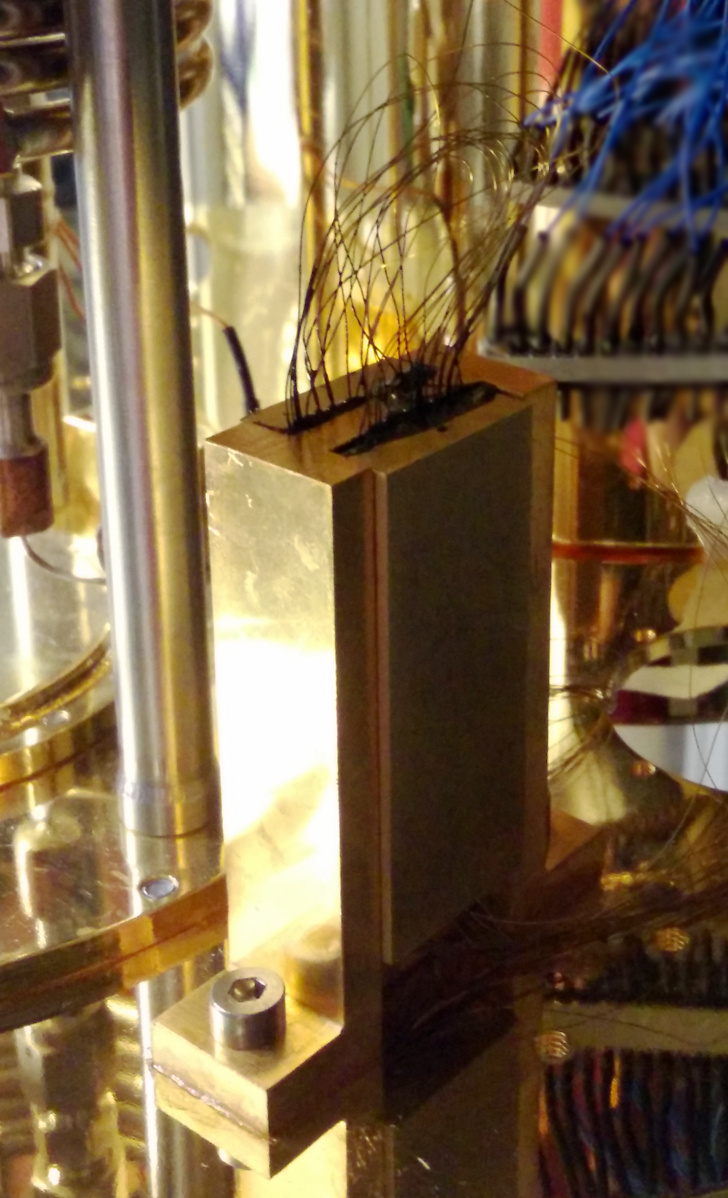
\includegraphics[height=1.2\textwidth]{Images/Thermalisation/DC}
        \caption{Fils de Manganin "stycastés" dans une presse dorée}
    \end{subfigure}%
    ~ 
    \begin{subfigure}[t]{0.48\textwidth}
        \centering
        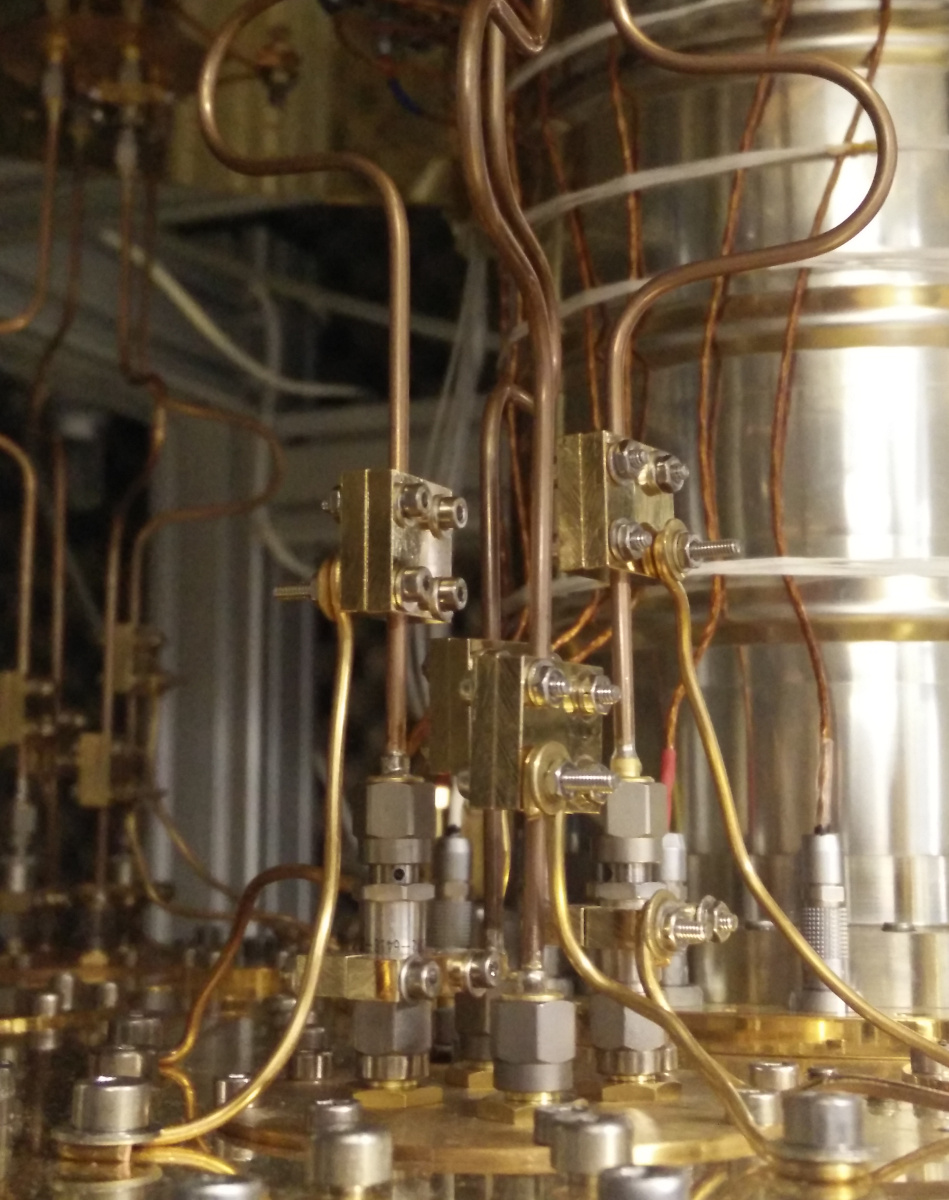
\includegraphics[height=1.2\textwidth]{Images/Thermalisation/Coax}
        \caption{Câbles coaxiaux thermalisés}
    \end{subfigure}
    \caption{Thermalisation des câbles sur la platine du cryostat}
\end{figure*}

\newpage
\section{Filtrage des lignes DC}
En plus de la thermalisation, les lignes DC sont filtrées à l'étage 20mK. Un premier filtrage est effectué dans le boîtier de thermalisation à l'aide d'un filtre Passe-Bas RC du second ordre.

\begin{figure}[h]
    \begin{center}
        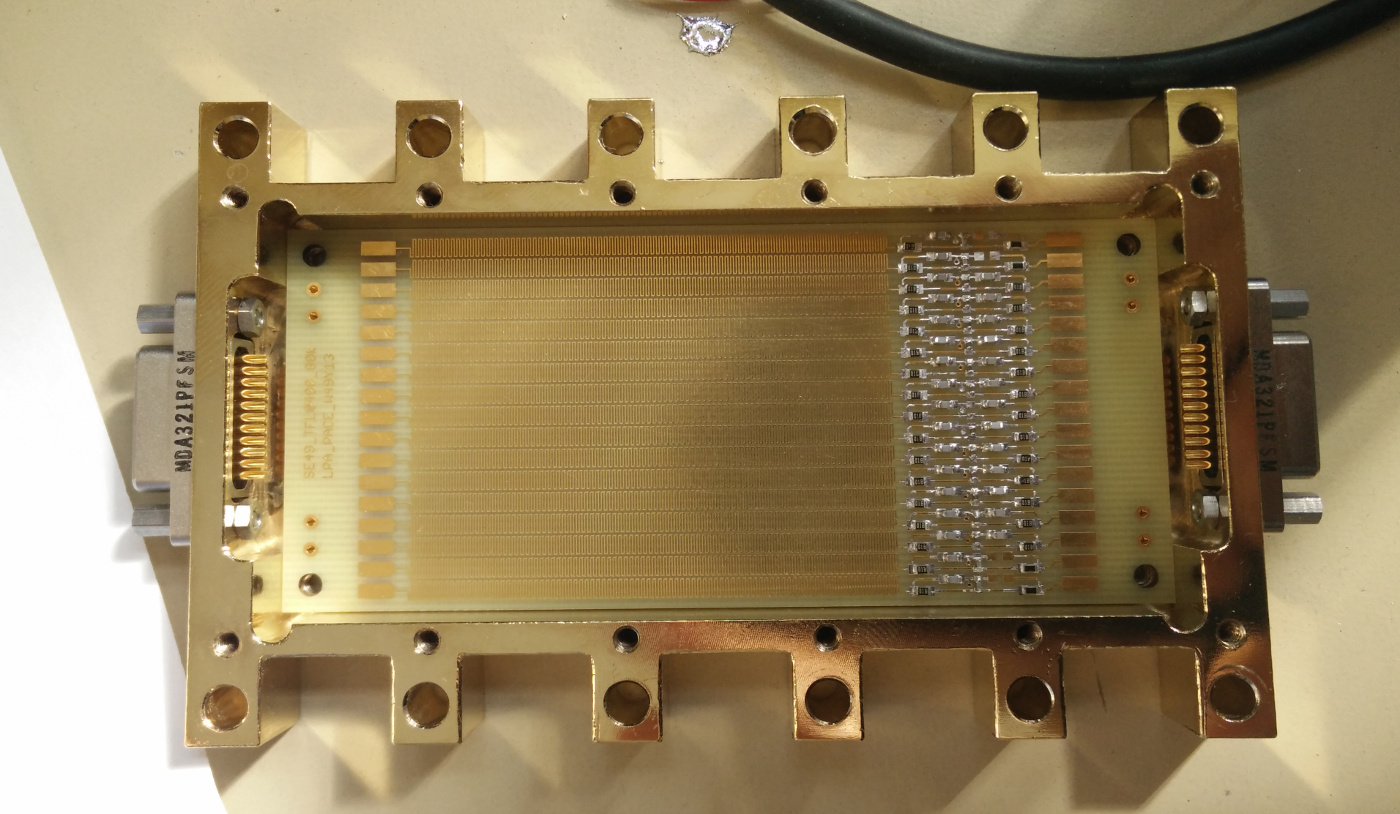
\includegraphics[height=0.4\textwidth]{Images/Thermalisation/DC3}
        \caption{Boîtier de thermalisation non soudé}
        \label{DC_Filtrage}
    \end{center}
\end{figure}

Un second filtrage est effectué grâce à l'Eccosorb. Cette résine composite à base d'époxy (même fabricant que la Stycast, mêmes solutions) absorbe très efficacement les micro-ondes résultant du bruit électronique.

Il a donc fallu mettre en place un petit boîtier, dans lequel nous faisons passer 17 câbles bleus de 80cm, compartimenté pour que l'Eccosorb n'abîme pas les prises lors du durcissement et des cycles de refroidissement.

J'ai donc décidé de dessiner des pièces en 3D sous OpenSCAD afin de former ces compartiments. Après quelques recherches, il est apparu que le matériau le plus utilisé en impression 3D, le PLA, peut être utilisé dans un cryostat (bien que jamais utilisé jusqu'ici).
\newline

En fait, beaucoup de matériaux ne sont pas compatibles avec de telles applications. Notamment, la faible pression dans le cryostat peut faire dégazer les matériaux (air dans les parois poreuses, ou des composants du matériau lui-même qui s'évapore). La plupart des matériaux élastiques sont dans ce cas.

De plus, certains matériaux peuvent ne pas supporter les cycles de refroidissement dans le cryostat. C'était le cas des précédentes séparations, qui ont alors cassé les câbles qui passaient au travers.

\subsection{Blindage des câbles DC}
En aval du boîtier de thermalisation, les câbles sont bien thermalisés et déjà bien filtrés. On ne voudrait donc pas laisser les câbles DC non blindés, au risque de recevoir des radiations, ne serait-ce que de l'étage à 100mK.

Une tresse métallique soudée à la masse entoure donc les câbles jusqu'au boîtier de filtrage micro-ondes. Celui-ci est directement branché sur la chambre d'expérience, les câbles restent donc isolés.

\begin{figure*}[t!]
    \centering
    \begin{subfigure}[t]{0.59\textwidth}
        \centering
        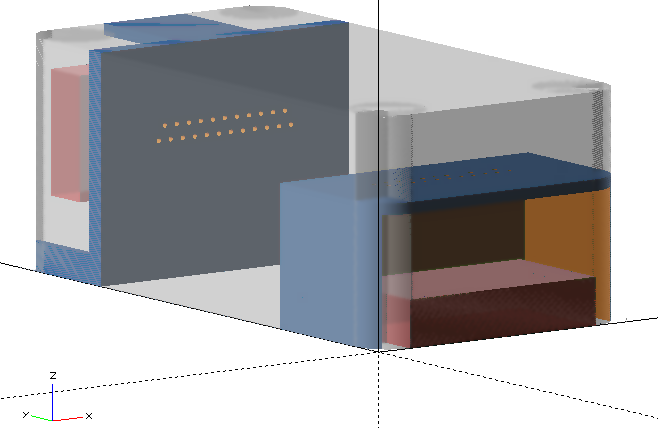
\includegraphics[height=0.633\textwidth]{Images/Thermalisation/Filtrage3D}
        \caption{Modélisation 3D des pièces dans le boîtier}
    \end{subfigure}%
    ~ 
    \begin{subfigure}[t]{0.39\textwidth}
        \centering
        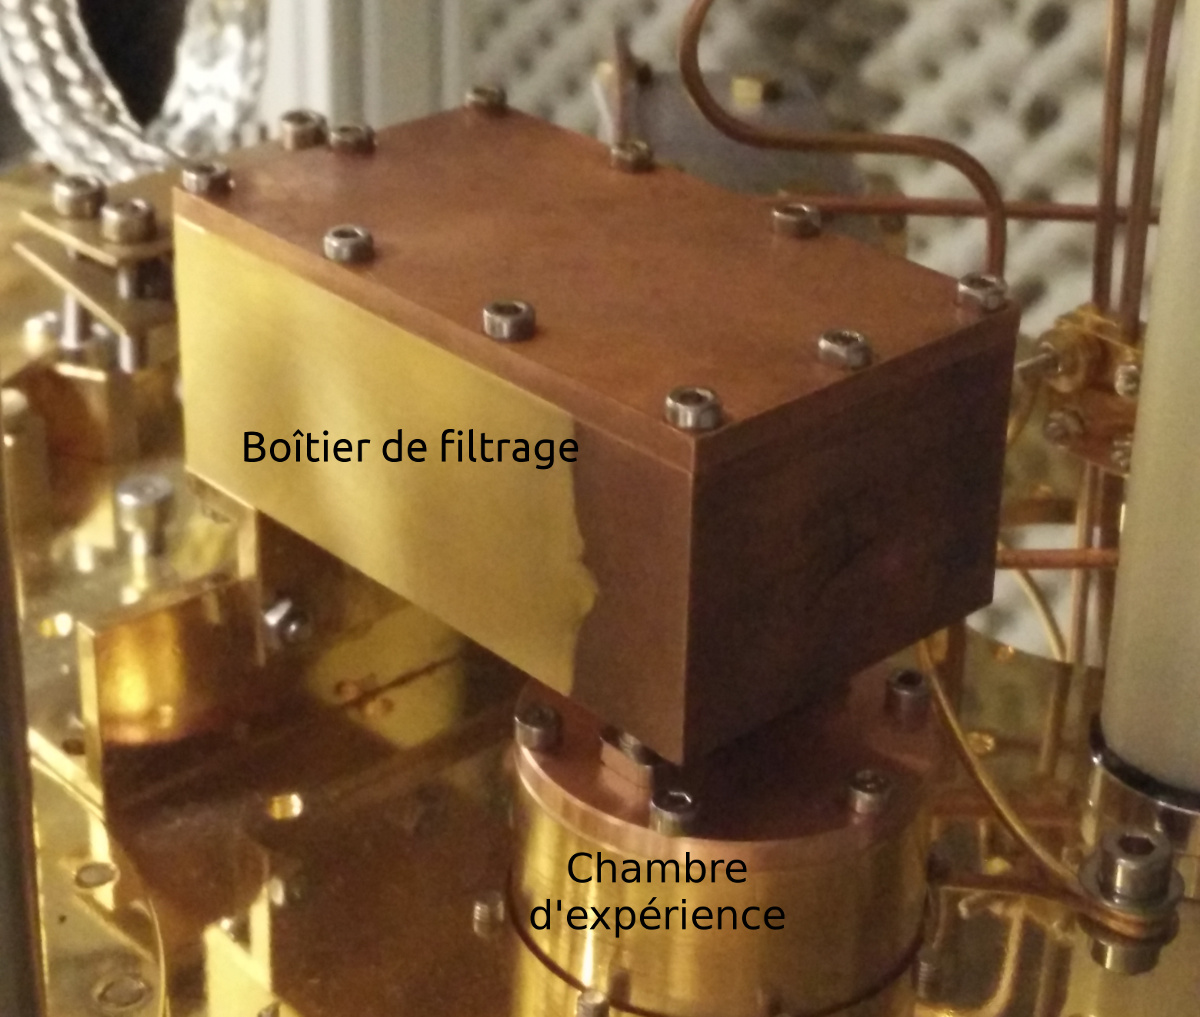
\includegraphics[height=0.95\textwidth]{Images/Thermalisation/Filtrage}
        \caption{Boîtier de filtrage en place dans le cryostat}
    \end{subfigure}
    \caption{Boîtier de filtrage, rempli d'Eccosorb}
\end{figure*}





\section{Fabrication des câbles coaxiaux}
Comme je l'ai précisé plus haut, les signaux RF sont véhiculés par des câbles coaxiaux semi-rigides. J'ai donc procédé intégralement à la fabrication et la caractérisation de ces câbles.
\newline

La moindre imperfection des câbles coaxiaux se ressent fortement sur leur atténuation -- nous verrons cela plus tard -- , il faut donc les manier et les cintrer en faisant attention à ne pas les tordre.

\subsection{Étapes de fabrication}
Je vais ici décrire les différentes étapes de fabrication d'un câble coaxial connectorisé. Elles peuvent être trouvées en annexe dans le guide de câblage.

\paragraph*{Dénudage} Il faut dénuder quelques millimètres du câble pour souder la pin sur l’âme du
câble coaxial, à l'aide d'une petite scie.
\begin{figure}[h]
    \begin{center}
        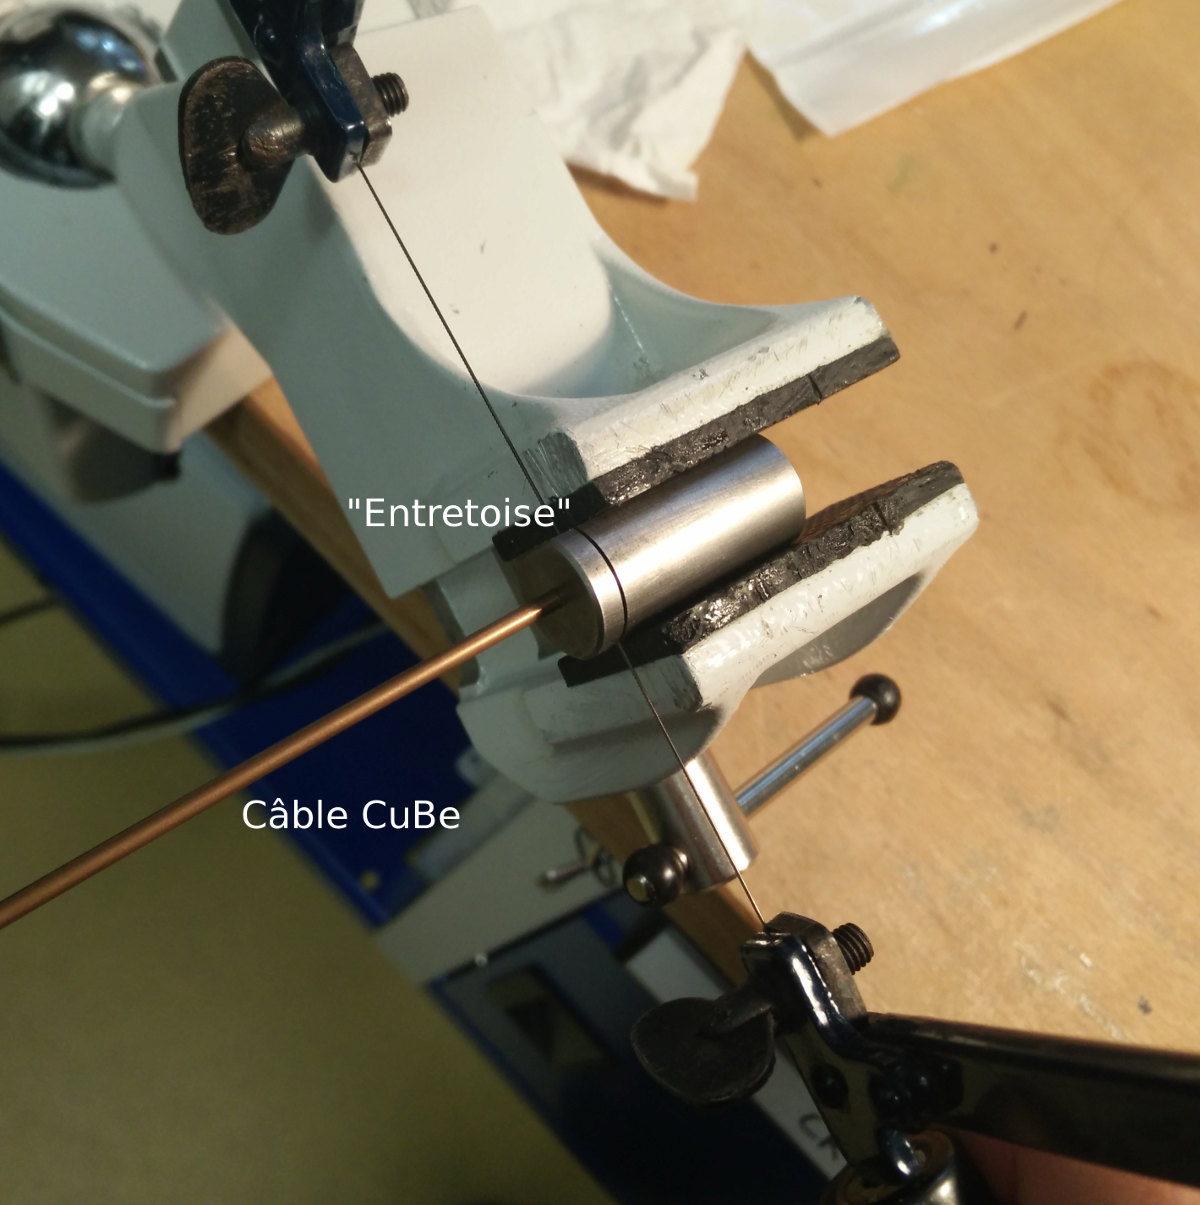
\includegraphics[height=0.48\textwidth]{Images/Coax/1}
        \quad
        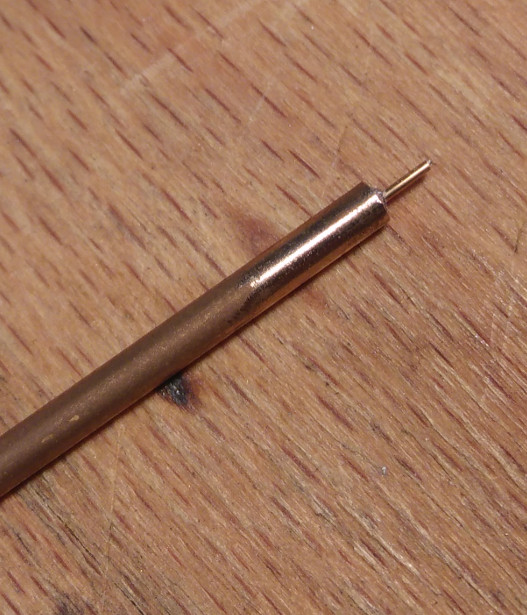
\includegraphics[height=0.48\textwidth]{Images/Coax/2}
        \caption{Dénudage d'un câble coaxial}
        \label{coax_denudage}
    \end{center}
\end{figure}

\paragraph*{Soudure de la pin centrale} On fixe une broche sur l’âme du câble, puis on serre le tout en
place. Pour prévoir la dilatation du diélectrique lors de la soudure, on place une petite entretoise juste avant la broche.
\begin{figure}[h]
    \begin{center}
        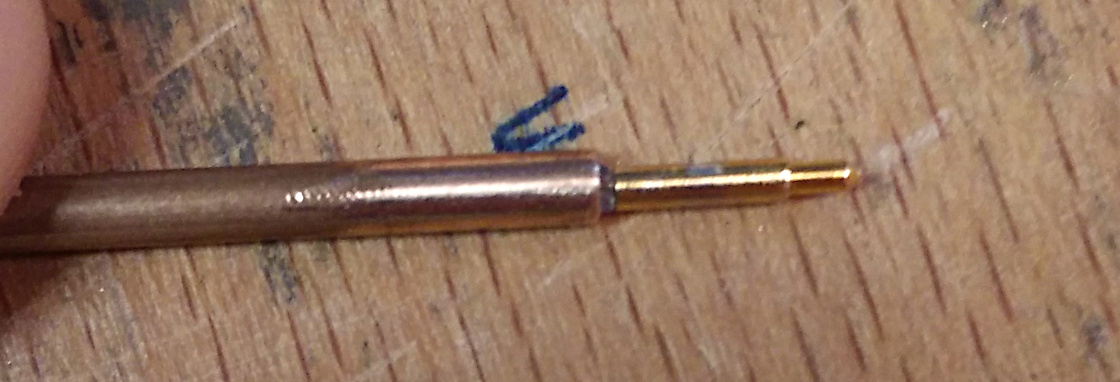
\includegraphics[width=0.60\textwidth]{Images/Coax/3}
        \caption{Pin centrale soudée sur le câble}
        \label{coax_soudure_centre}
    \end{center}
\end{figure}

\paragraph*{Soudure de la prise extérieure} On fixe sur la prise mâle une prise femelle factice qui permet de positionner à la distance correcte la prise mâle. Celle-ci a une partie mobile avec le pas de vis.
\begin{figure}[ht]
    \begin{center}
        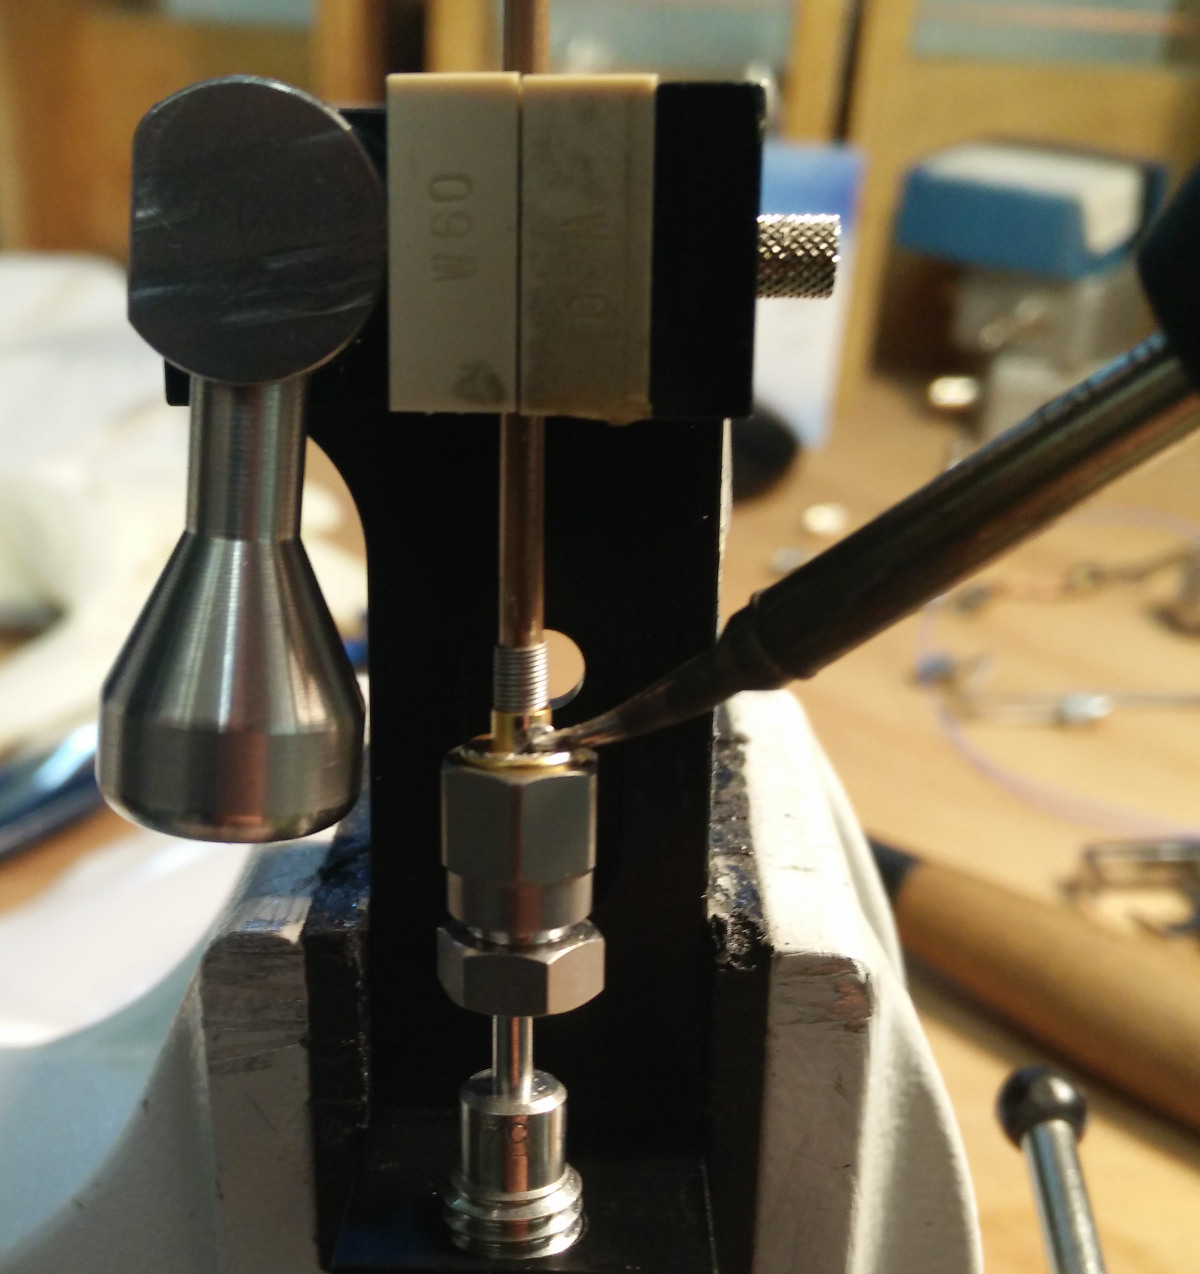
\includegraphics[height=0.48\textwidth]{Images/Coax/4}
        \quad
        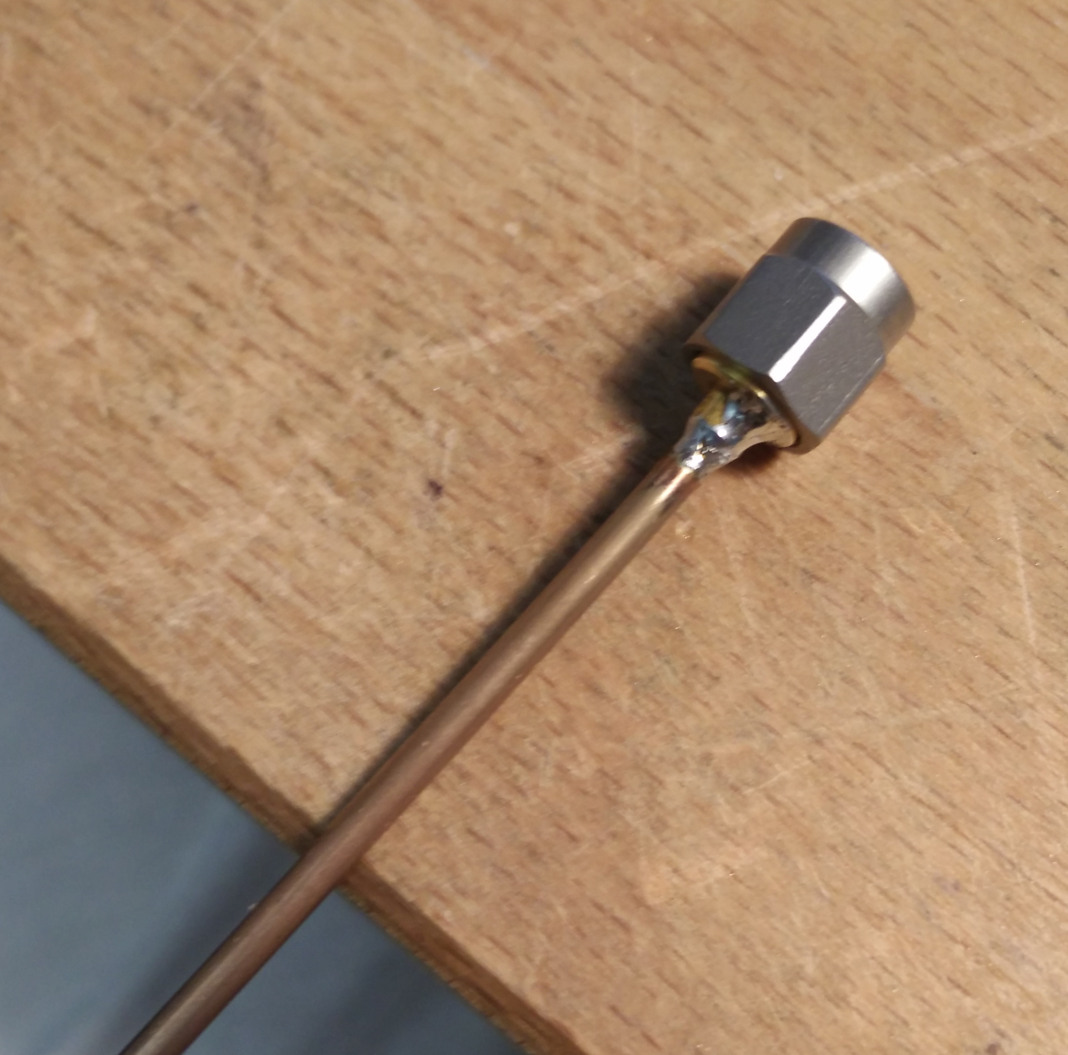
\includegraphics[height=0.48\textwidth]{Images/Coax/5}
        \caption{Soudure de la prise extérieure}
        \label{coax_soudure_exterieur}
    \end{center}
\end{figure}

\paragraph*{Fixation de l’isolant}  La dernière étape est de mettre un petit cylindre diélectrique entre la prise et la broche. On utilise alors une pièce creuse qui se visse dans le connecteur pour enfoncer le diélectrique.

\begin{figure}[ht]
    \begin{center}
        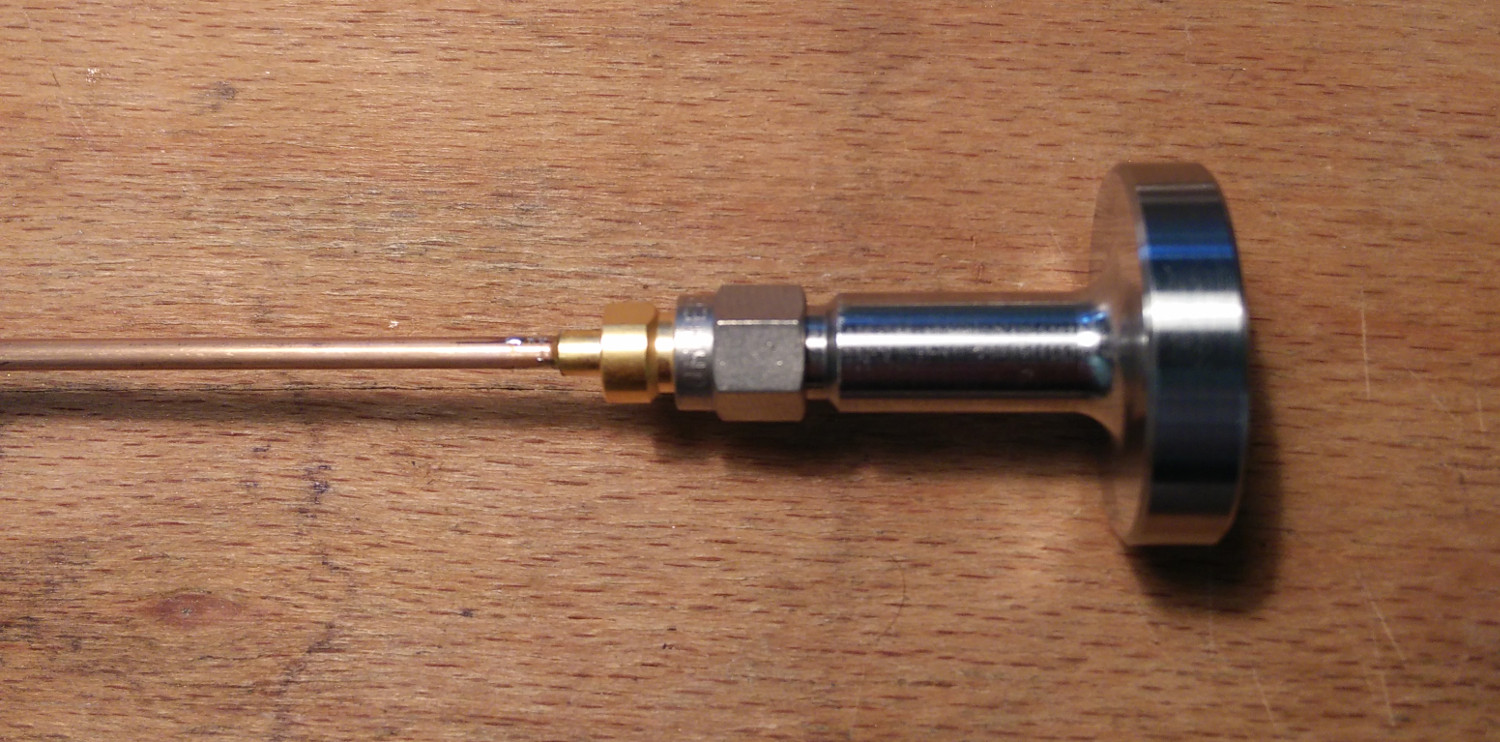
\includegraphics[width=0.60\textwidth]{Images/Coax/6}
        \caption{Fixation de l’isolant}
        \label{coax_fixation_isolant}
    \end{center}
\end{figure}

\paragraph*{Mesure du câble nécessaire} Après avoir connectorisé une extrémité du câble, il faut mesurer précisément la longueur de câble nécessaire. Il faut alors prendre en compte la longueur de câble qui se trouve dans le connecteur (sinon, il manquera quelques millimètres).

\begin{center}
    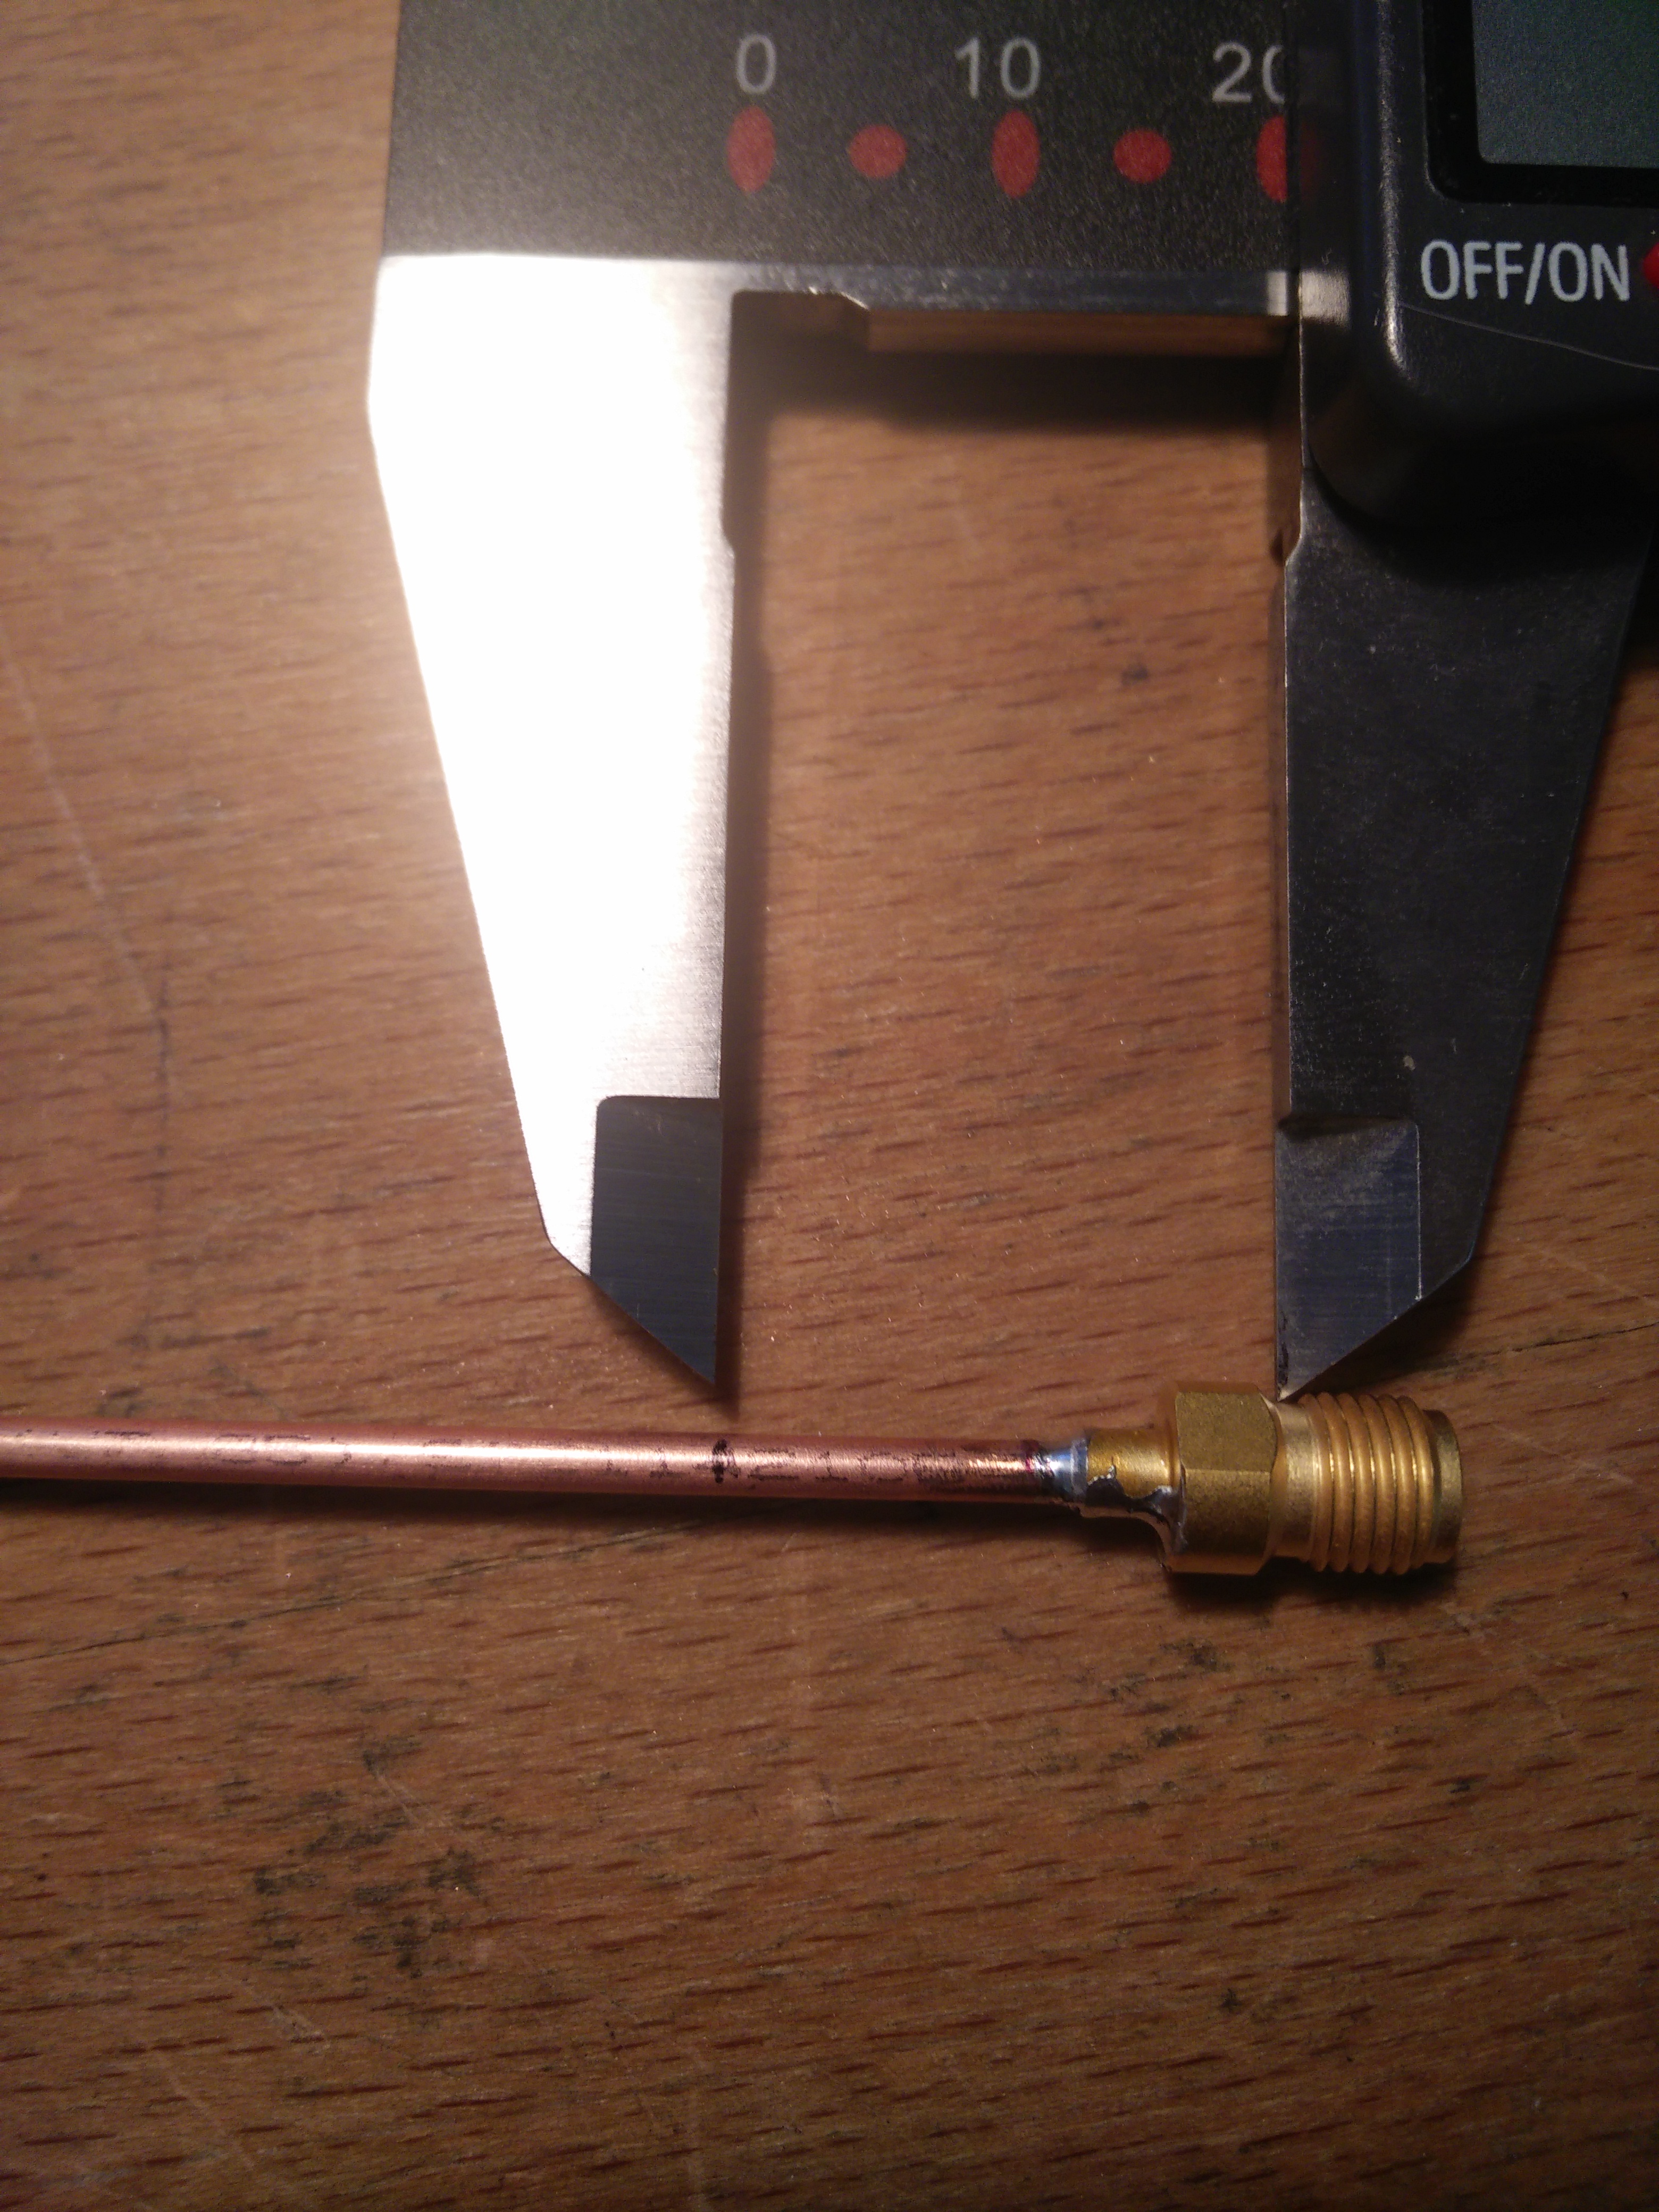
\includegraphics[width=0.40\textwidth]{Images/Coax/mesure}
    \label{coax_mesure}
\end{center}

\newpage
\paragraph*{Cintrage des câbles coaxiaux} Comme évoqué plus haut, les câbles doivent être cintrés entre chaque étage du cryostat. Néanmoins la fragilité des câbles nous impose de respecter un rayon de courbure minimal de 9mm.

Une cintreuse "sur mesure" permet de cintrer les câble correctement.

Pour les mesures, il faut prendre en compte 28mm de câble pour faire un demi-tour. Un cintrage en "U" nécessite alors 35mm de câble de plus qu'un câble droit.

\begin{figure}[h]
    \begin{center}
        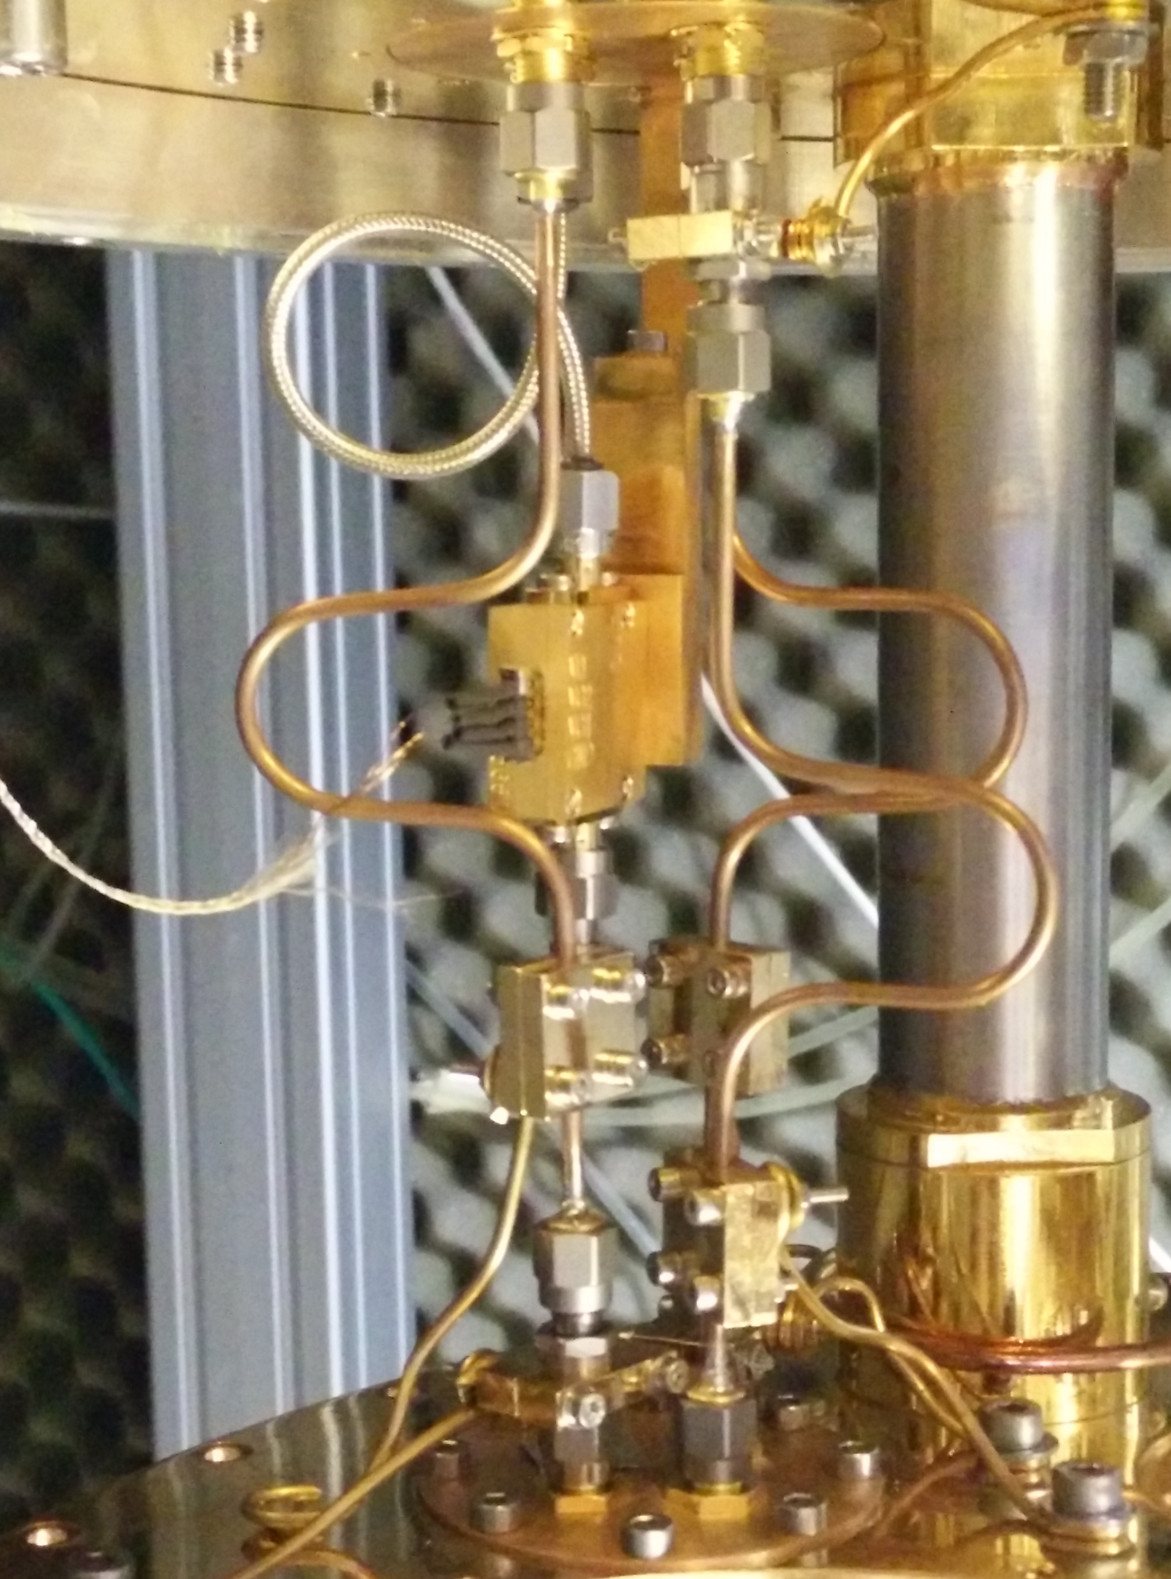
\includegraphics[width=0.60\textwidth]{Images/Coax/cintrage}
        \caption{Câbles coaxiaux cintrés en "U" et connectés}
        \label{coax_cintrage}
    \end{center}
\end{figure}




\chapter{Caractérisation des câbles coaxiaux}

Maintenant que les câbles ont été cintrés et connectorisés, il faut mesurer leur caractéristique atténuation/fréquence. D'une part pour vérifier si les câbles sont utilisables, et d'autre part pour avoir les valeurs exactes d'atténuation afin de calibrer nos mesures à fréquence fixée.

L'appareil dédié à cette tâche est le VNA (Vector Network Analyzer) ou PNA (Performance Network Analyzer). L'équipe a récemment fait l'acquisition d'un PNA N5242 de Agilent.

Les graphes obtenus représentent l'atténuation en dB, qui est l'unité de mesure habituelle pour les câbles coaxiaux.
%TODO Finir le paragraphe
\begin{figure}[h]
    \begin{center}
        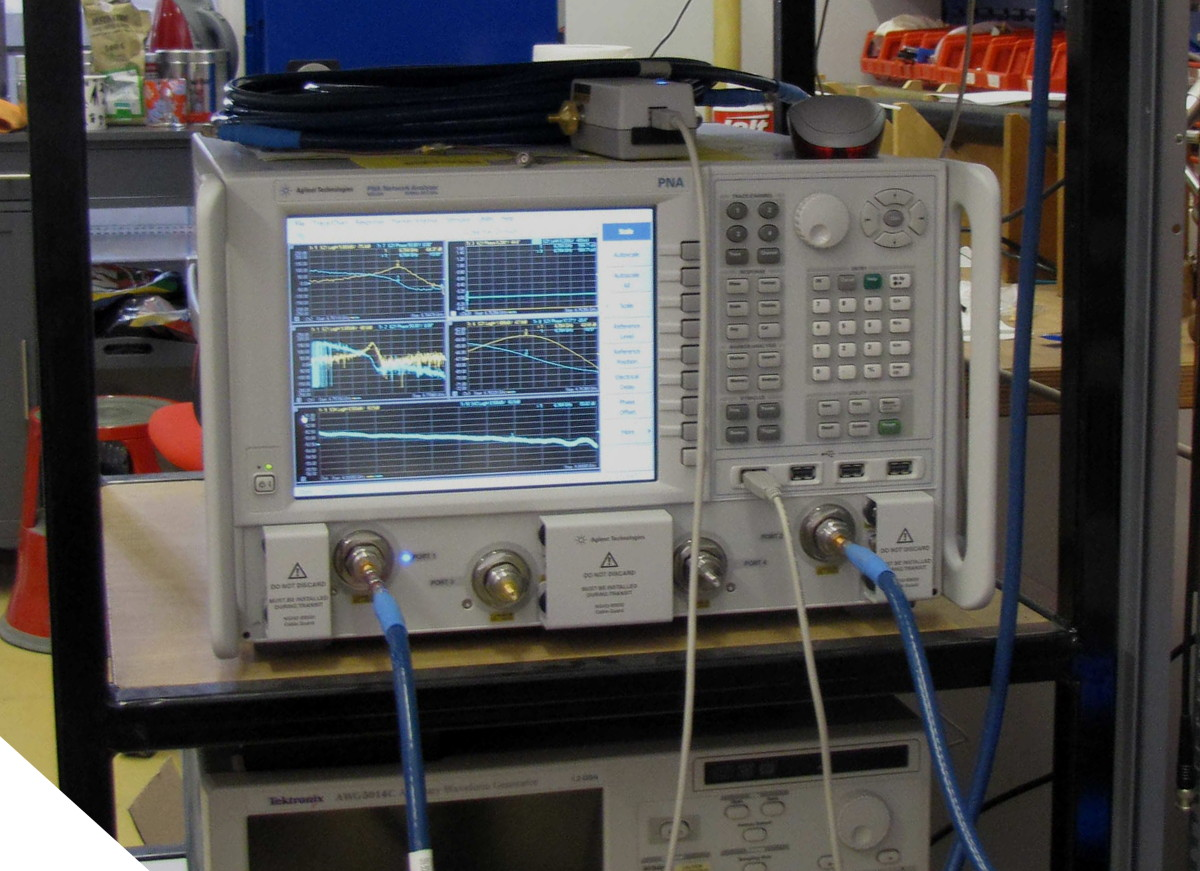
\includegraphics[width=0.65\textwidth]{Images/VNA}
        \caption{Le PNA de l'équipe}
        \label{PNA}
    \end{center}
\end{figure}

En se plaçant sur un canal de mesure, on effectue une calibration électronique (à l'aide d'un boîtier externe connecté au PNA) avec les câbles flexibles supplémentaires, puis on connecte notre câble coaxial.

\newpage
\section{Paramètres du PNA}
\begin{description}
    \item[Gamme de mesure :] 1GHz - 20GHz et 4-8GHz
    \item[Nombre de points :] 12801
    \item[Puissance :] -20dB et Power On
    \item[IF Bandwidth :] 1kHz
\end{description}

On effectue deux séries de mesure, entre 1 et 20GHz et entre 4 et 8GHz.

\section{Résultats attendus}

\begin{itemize}
    \item L'atténuation augmente avec la fréquence
    \item Elle est comprise entre -0.5dB et -2.5dB
    \item Jusqu'à 8GHz, l'atténuation doit être assez stable (peu de sinusoïdale) : L'essentiel des mesures est effectée entre 4 et 8GHz, d'où la série de mesures restreinte à cette gamme.
\end{itemize}

\begin{figure}[ht]
    \begin{center}
        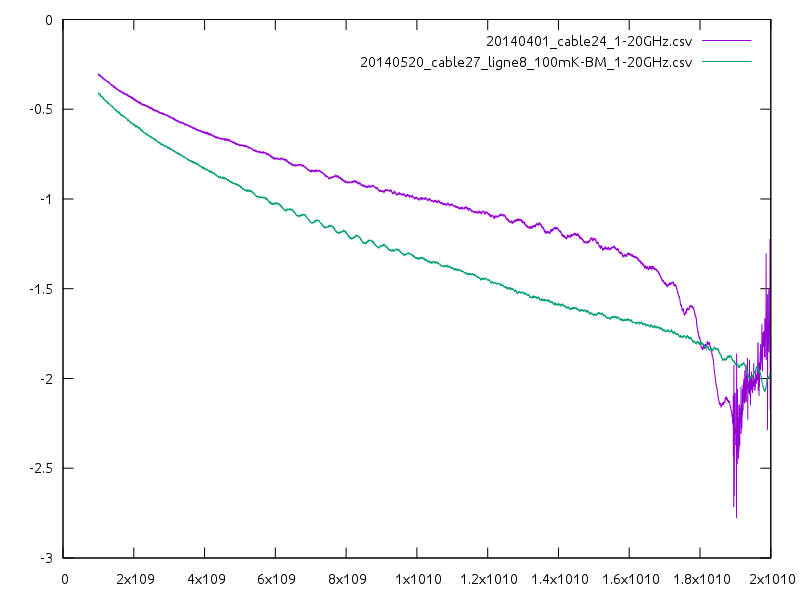
\includegraphics[width=0.65\textwidth]{Images/Caracs/abime2.png}
        \caption{La caractéristique d'un câble correct(vert) et un abîmé (violet)}
        \label{Carac1}
    \end{center}
\end{figure}

Néanmoins un câble très cintré n'est pas forcément synonyme de mauvaise caractéristique.


\begin{figure*}[ht]
    \centering
    \begin{subfigure}[t]{0.40\textwidth}
        \centering
        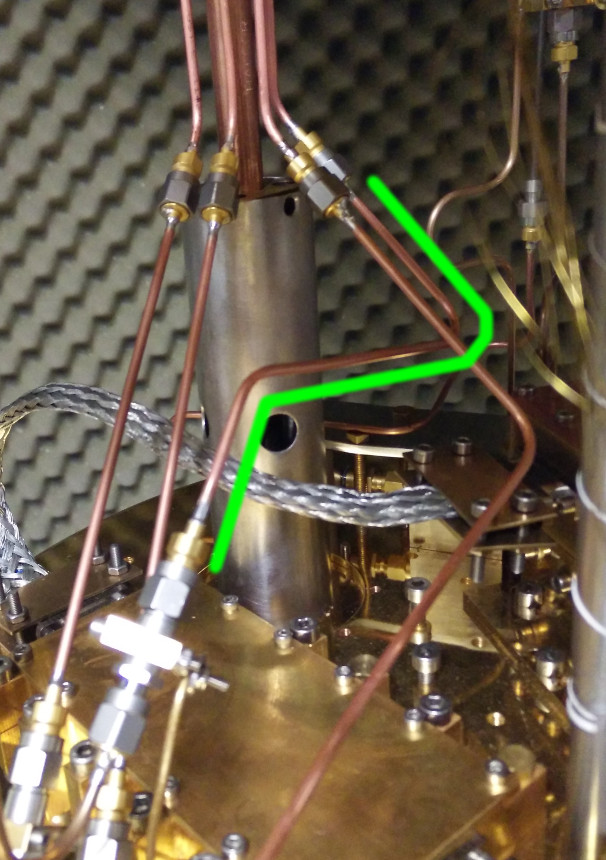
\includegraphics[height=1.2\textwidth]{Images/Coax/Tres_cintre}
        \caption{Câble cintré à plus de 270\textdegree }
    \end{subfigure}%
    \begin{subfigure}[t]{0.6\textwidth}
        \centering
        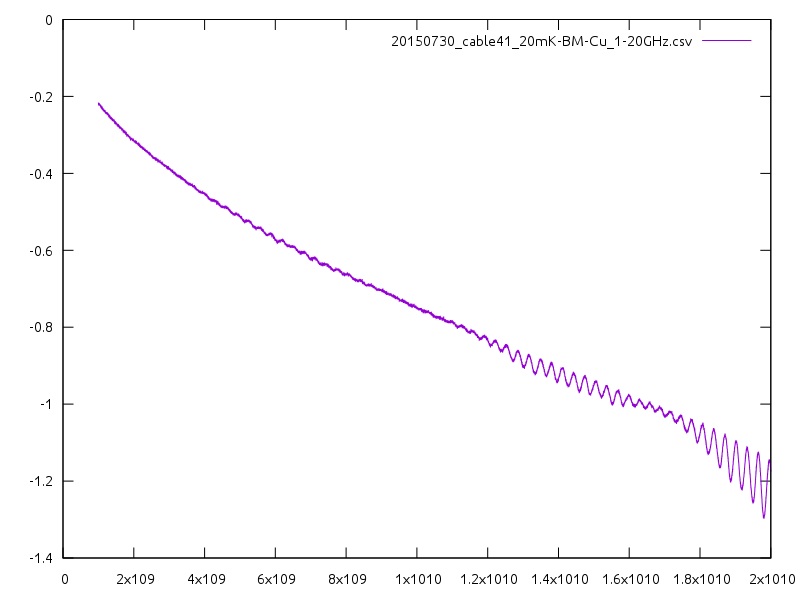
\includegraphics[width=1.0\textwidth]{Images/Caracs/Tres_cintre}
        \caption{Caractéristique très bonne}
    \end{subfigure}
    \caption{Câble très cintré à bonne caractéristique}
\end{figure*}


\newpage
\section{Guide de câblage}
En complément du travail de câblage que j'ai effectué, j'ai écrit un guide de câblage détaillant les étapes à suivre afin de connectoriser un câble coaxial, ainsi que pour le caractériser.\newline

Celui-ci se trouve en annexe. Il détaille aussi la mise en place des boîtier de filtrage et l'utilisation du VNA.







\chapter*{Bilan}
\addcontentsline{toc}{chapter}{Bilan}

L'expérience a donc pu être câblée intégralement, malgré quelques aléas qui ont retardé l'installation de la bobine par CryoConcept.

J'ai malheureusement quitté le laboratoire avant de pouvoir finir le montage à l'intérieur du cryostat -- les câbles étaient néanmoins assemblés et les pinces de thermalisation en place à l'extérieur --, mais j'ai pu fournir un guide de câblage complet.\newline

De nouvelles expériences n'ont pas encore été effectuées avec les nouveaux câbles, je ne peux donc pour le moment présenter comme résultats de mesures que les caractéristiques des câbles que j'ai fabriqués qui sont largement acceptables.\newline

Ce stage a été une opportunité pour moi de découvrir l'environnement des laboratoires de recherche, que nous n'avons pu apercevoir que rapidement pendant notre projet de recherche. Outre ma mission principale, j'ai pu m'intégrer à l'équipe Hybrid Quantum Circuits et comprendre les différents thèmes gravitant autour de la spintronique et l'étude des nanotubes de carbone.\newline

Enfin, ce stage m'a permis de mieux appréhender les problèmes expérimentaux qui peuvent se présenter, leurs solutions techniques ainsi que les limites auxquelles nous pouvons être confrontés.\newline

Bien que je n'aie pas eu l'occasion de mettre  en application de façon apparente mes connaissances en physique durant mon stage, j'ai pu les enrichir par mon implication dans l'équipe. J'ai notamment observé le comportement d'un séparateur à paires de Cooper, ou l'effet Kondo par couplage des électrodes et du nanotube de carbone.

\bibliographystyle{unsrt}
\bibliography{bibliographie}
\listoffigures
\newpage
\appendix
\phantomsection
\addcontentsline{toc}{part}{Annexes}

\vspace*{8cm}
\begin{center}
\rule{\linewidth}{0.5mm}\\[0.7cm]
{\huge{\bfseries Annexes}}\\[0.4cm]
\rule{\linewidth}{0.5mm}\\[0.5cm]


\end{center}
\newpage
\phantomsection
\addcontentsline{toc}{chapter}{Guide de câblage du cryostat}
\includepdf[pages={-}]{../guide.pdf}
\end{document}
